\jxhj{%教学后记
	}
\skrq{%授课日期
	2017年12月21日 4-5节}
\ktmq{%课题名称
	 局部坐标系}
\jxmb{%教学目标,每行前面要加 \item
	\item 掌握Fanuc上G52指令的格式;
	\item 掌握Siemens上Trans指令的格式;
	\item 掌握用局部坐标系指令编程。
}
\jxzd{%教学重点,每行前面要加 \item
	\item 掌握Fanuc上G52指令的格式;
	\item 掌握用局部坐标系指令编程。 }
\jxnd{%教学难点,每行前面要加 \item
	\item 掌握用局部坐标系指令编程。 }
\jjff{%教学方法
	通过讲述、举例、演示法来说明;}

\makeshouye %制作教案首页

%%%%教学内容
\subsection{组织教学}
\begin{enumerate}[\hspace{2em}1、]
	\item 集中学生注意力;
	\item 清查学生人数;
	\item 维持课堂纪律;
\end{enumerate}

\subsection{复习导入及主要内容}
\begin{enumerate}[1、]
\item Fanuc上的倒角、倒圆角的指令格式;
\item Siemens上的倒角、倒圆角的指令格式;
\item 编程实例。
\end{enumerate}

\subsection{教学内容及过程}
\subsubsection{几种坐标系}
	1、工件坐标系:G54-G59、G92
	
	G54-G59是在机床参数中以机床坐标为基准设定工件坐标系

	G92是在程序中以刀具当前位置为基准设定工件坐标系

	一般使用G54~G59指令后,就不再使用G92指令。

	2、机床坐标系:G53

	当需要用机床坐标系编程时,用G53指令。

	机床坐标系通过回零(回参考点)建立。

	如坐标系不对,可通过回零重新建立机床坐标系,机床坐标系原点在机床上是固定的一个点,这个点不会变的。

	3、局部坐标系:G52、Trans

	在工件坐标上建立一个子工件坐标系。即局部坐标系。


\subsubsection{Fanuc上局部坐标系}
	指令格式:  G52 X\_ Y\_ Z\_;建立局部坐标系

	G52 X0 Y0 Z0 ;取消局部坐标系。

	说明:其X、Y的定义是原坐标系的程序原点到子坐标系的程序原点之向量值。

	G52 X0 Y0;=>表示回复到原坐标系。

	注意:

	1、局部坐标系设定不改变工件和机床坐标系。 

	2、当用G50定义工件坐标系时,如果没有对局部坐标系中的所有轴指定坐标值,局部坐标系保持不变。如果没有为局部坐标系中的任何轴指定坐标值,局部坐标系被取消。 

	3、G52暂时取消刀尖半径补偿中的偏移。 

	4、在绝对方式紧跟G52之后指令一个运动指令。 

	5、复位时是否取消局部坐标系取决于参数的设定。当3402号参数的第6位(CLR)或者1202号参数3位(RLC)设为1时,局部坐标系在复位状态被取消。 

	6、手动返回参考点是否取消局部坐标系取决于ZCL的设定(参数1201的第2位)。

\subsubsection{Siemens上的局部坐标系}

	指令格式:

	TRANS X\_ Y\_ Z\_ ;可编程的偏移,清除所有有关偏移、旋转、比例系数、镜像的指令 

	ATRANS X\_ Y\_ Z\_ ;可编程的偏移,附加于当前的指令 

	TRANS;不带数值清除所有有关偏移、旋转、比例系数、镜像的指令 

	TRANS/ATRANS 指令要求一个独立的程序段。

	四、编程实例:

	在数控机床上加工如图所示的零件,完成工艺分析及加工程序的编写。
	
	\begin{figure}
		\centering
		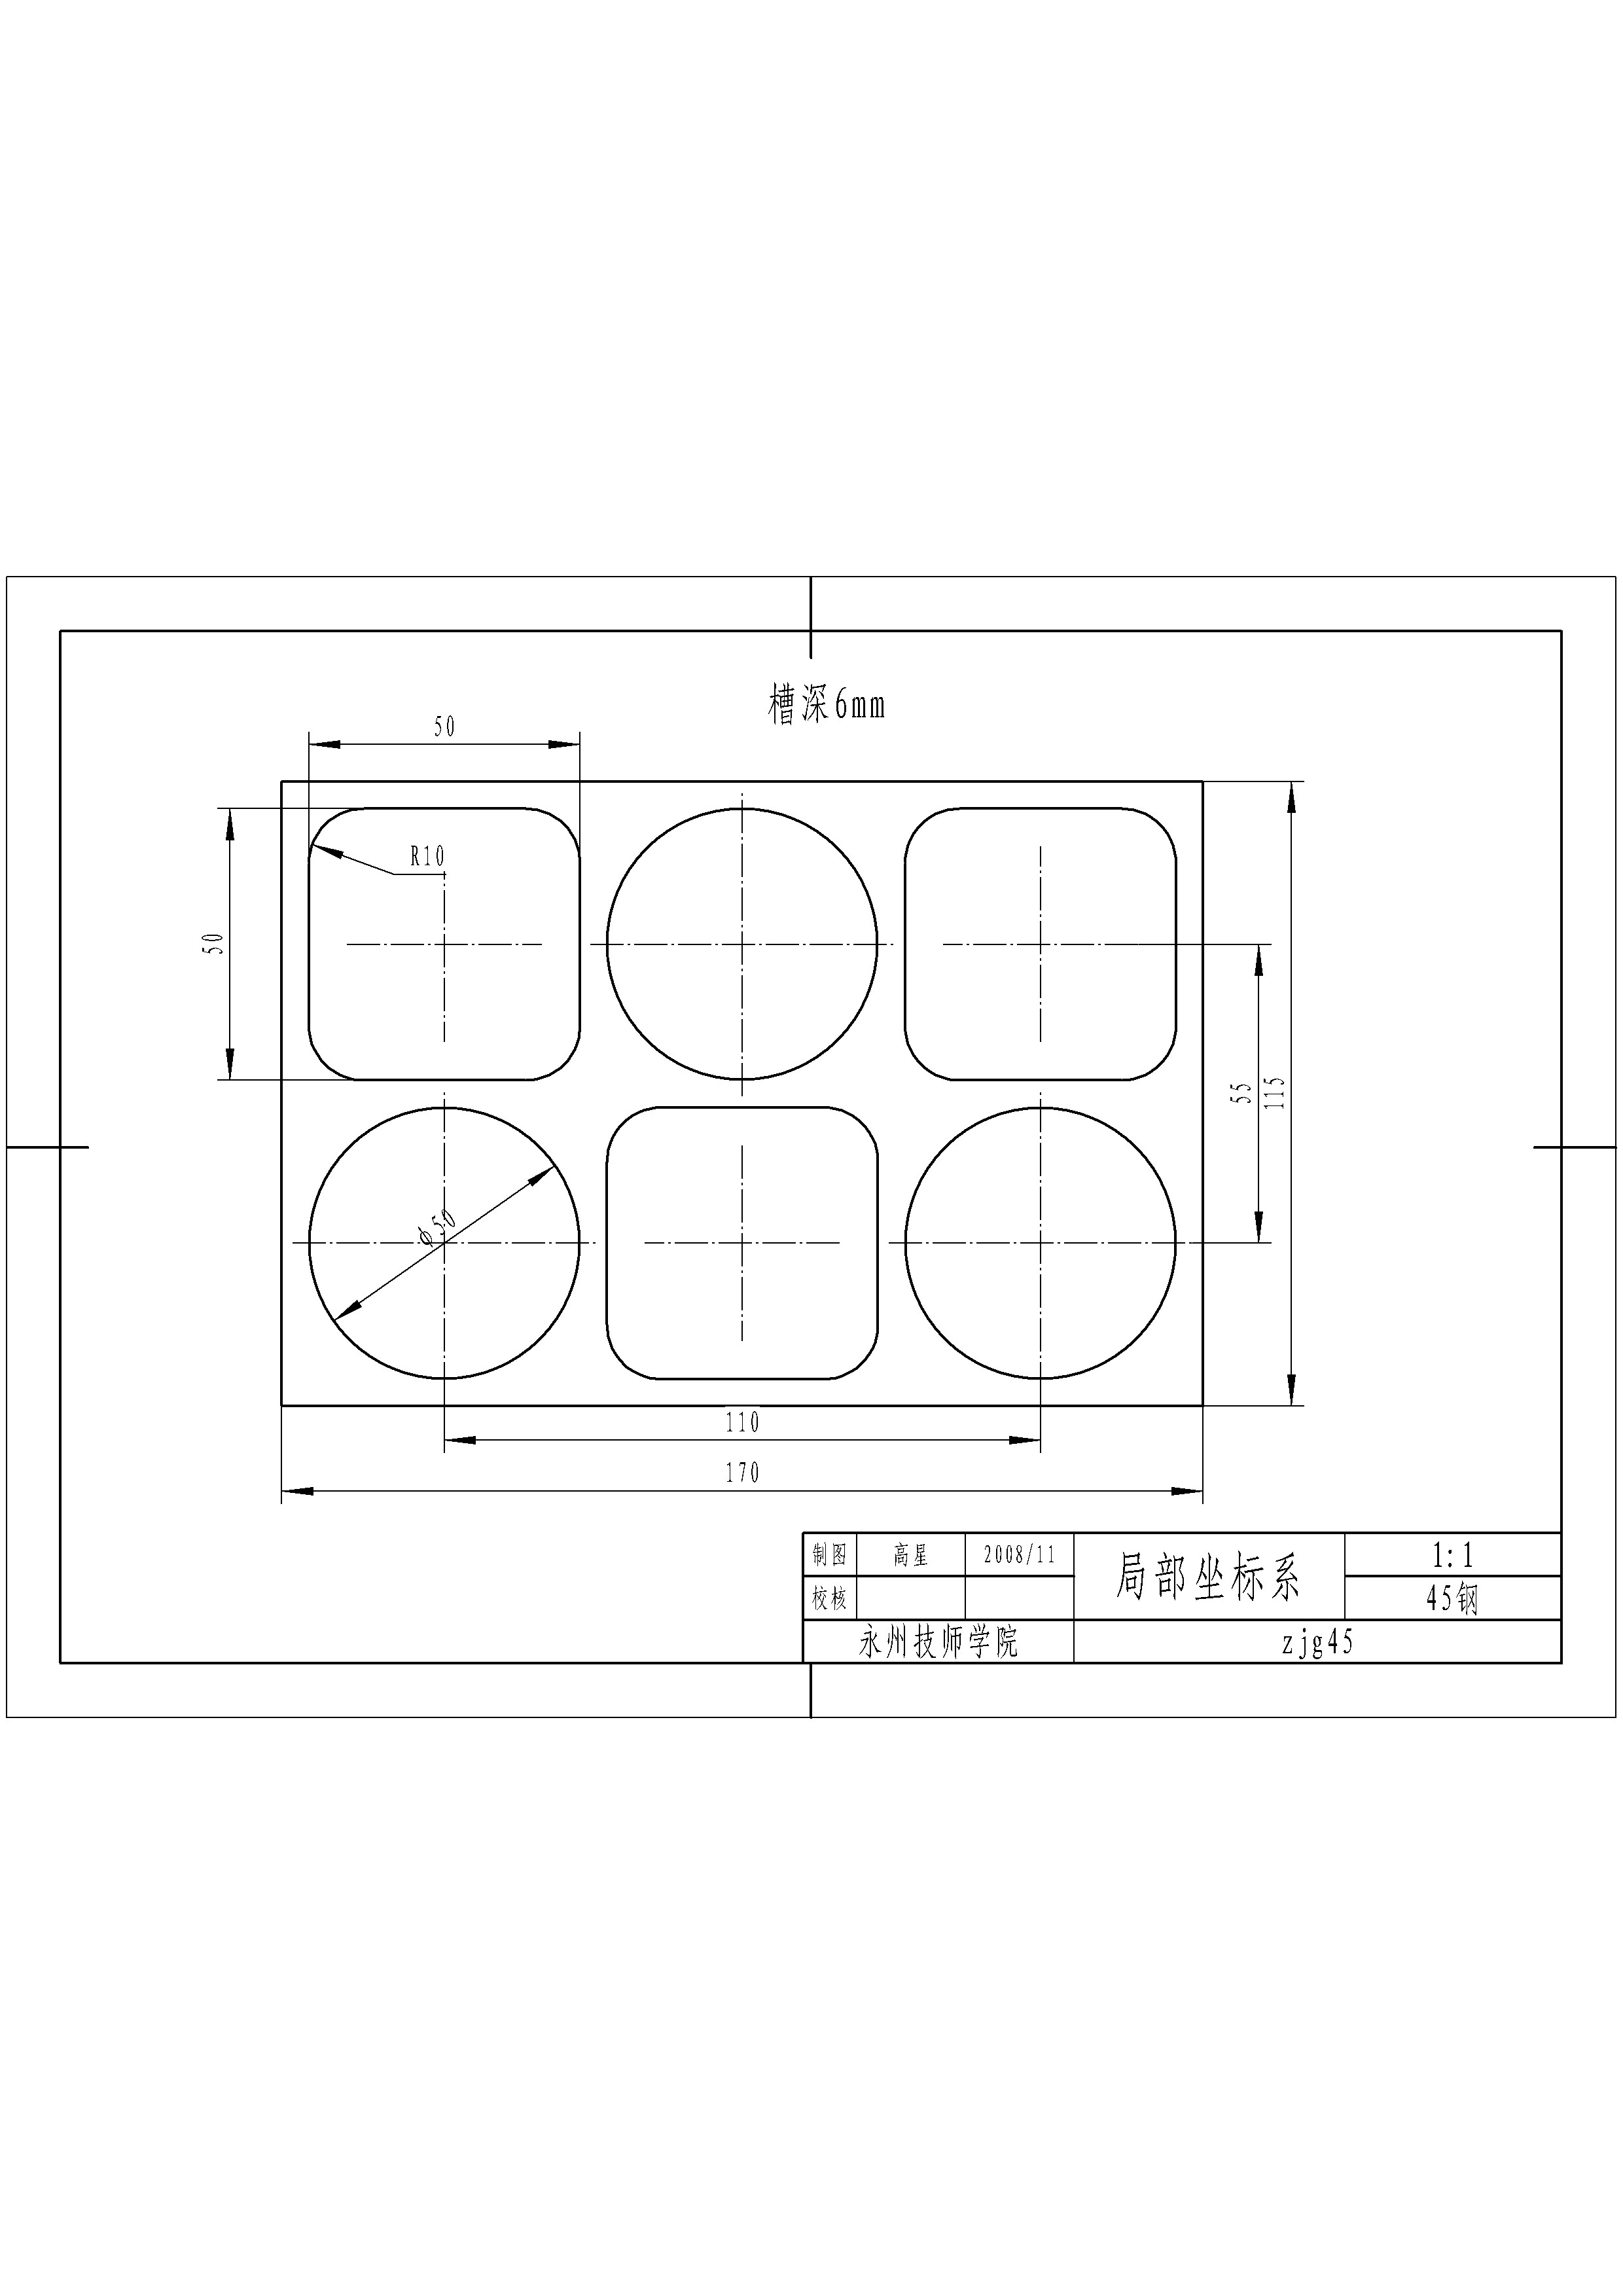
\includegraphics[width=0.9\linewidth,trim=50 285 50  250,clip]{data/image/29-1}
		\caption{加工实例}
		\label{fig:29-1}
	\end{figure}

1、工件坐标系:

2、装夹

3、刀具:

$\varnothing$12立铣刀

$\varnothing$8立铣刀

4、加工顺序

	
\subsubsection{如图\ref{fig:29-2}所示,加工40*40矩形凸台,高3mm,刀具为Ф14的平底刀。}

	\begin{figure}
	\centering
	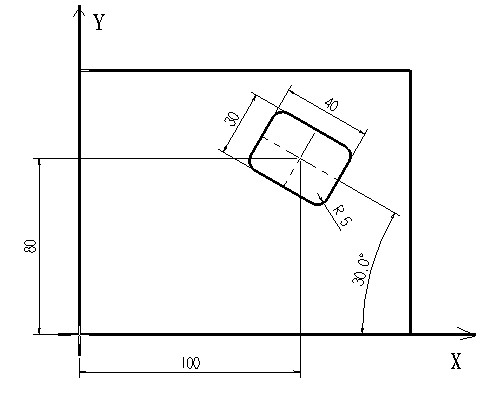
\includegraphics[width=0.9\linewidth,trim=0 0 0 0,clip]{data/image/29-2}
	\caption{加工实例}
	\label{fig:29-2}
\end{figure}

分析:

(1)凸台为倾斜形式,可以使用旋转指令编程。

(2)凸台四角带圆角,可以使用倒圆角指令编程。

(3)使用局部坐标系,将当前工件坐标系移至凸台的中心处。

加工程序如下:

\begin{lstlisting}
O1(FANUC)
G54G17G90G40
G01Z100F2000
M03S500
G52X100Y80            当前工件坐标系移至凸台的中心处
G68X0Y0R-30           当前工件坐标系顺时针旋转30度
G00X-35Y0
G01Z-3F1000            
G01G41X-30Y-10D01
G03X-20Y0R10
G01Y15,R5              倒圆角R5
X20,R5
Y-15,R5
X-20,R2
Y0
G03X-30Y10R10
G01G40X-35Y0
G01Z100F2000
G69                    取消坐标系旋转
G52X0Y0               取消坐标系平移
M05
M30
\end{lstlisting}


\subsection{课堂小结}
\begin{enumerate}[1、]
\item 几种坐标系;
\item Fanuc 上局部坐标系;
\item Siemens 上局部坐标系;
\item 编程实例。
\end{enumerate}

\vfill
\subsection{布置作业}
\begin{enumerate}[1、]
	\item 综合习题一。
\end{enumerate}
\vfill